\documentclass[12pt]{report}

\usepackage[margin=0.7in]{geometry}
\usepackage{graphicx, verbatim, listings, fancyvrb, color, float, pdfpages}
\usepackage[english]{babel}
\usepackage[autostyle]{csquotes}
\usepackage{dirtree}
\usepackage{titling}
\usepackage{graphicx}


\graphicspath{ {/Users/kim-anh/Documents/University/AIN/MDPPacman/report2/images/} }

\setlength{\droptitle}{-8em}   % This is your set screw

\title{6CCS3AIN Coursework: \\ Pacman in a hard(er) world}
\author{
  Kim-Anh Vu\\1707295\\
  \texttt{kim-anh.vu@kcl.ac.uk}
}
\date{November 2019}


\begin{document}
% Title page %
  \begin{titlepage}
    \maketitle
  \end{titlepage}
  \section*{Introduction}
    By implementing the MDP-solver and discovering the optimum values to set specific
    variables, the task was to be able to guide Pacman safely around the grid and
    win the game by consuming all of the food that is available.

    \section*{Implementation}

      \subsection*{Board Class}
        When the getAction() function in the MDPAgent class is called, the necessary information (current position, corners, food, ghosts, walls, legal, capsules) are assigned to local variables from the API provided.
        \newline \newline
        Firstly, to get the width and height of the layout, the corners list was used to find the maximum x and y value from the list of tuples and increment each value by 1. This is a better way of calculating the height and width than finding out which coordinates had the maximum y value and accessing the value directly using indexing, as order of the coordinates could change, so height and width values would not be accurate.
        \newline \newline
        Then, creating a separate Board class, which width, height and the reward value for non-terminal states (which will be the default reward value for each position on the board) is passed to. Then, set the reward of positions of the food, ghosts and capsules - replicating the layout of the board used. Also, rewards of positions surrounding the ghosts will have a value that is more than the reward of ghosts but lower than the reward value for non-terminal states. Walls do not get a reward, thus `x' is assigned to each wall position.
        \newline \newline
        Public functions were also created in the Board class to prevent other classes from accessing the board and its attributes directly, contributing to achieving loose coupling. Examples of functions that are in the Board class are setting values of each position and converting the y coordinates, as the board (represented as a nested list) has row 0 as the top row, whereas the actual layout of the game's rows started from the bottom and the y coordinate increases as you go up. Therefore, you need a function that will be able to convert y coordinates of one board/layout to another.
        \newline \newline
        To obtain the updated board with each state containing an utility value, the function calls on the value iteration function.

      \subsection*{Value Iteration}
        `board' will be used to obtain the original rewards for each position.
        \newline `board\_copy' contains the deepcopy of the board that has been passed into the value iteration function and is the board that is used to update the utility for each state.
        \newline `U' is the previous state of `board\_copy'
        \newline
        \newline \hspace*{1cm} \underline{Example:}
        \newline \hspace*{1cm} You have updated the value at (x, y) in `board\_copy' and you needed the value at (x, y + 1) \hspace*{1cm} to do so. Now you need to update the value at (x, y + 1), which will need the old value of (x, \hspace*{1cm} y) which will be stored in `U'.
        \newline \newline
        This function iterates through `board\_copy' for maximum of 15 times, resets the variable total\_difference (total difference between current board and future board) to zero and checks whether or not the cell is anything but a wall or a ghost. This is done by confirming if the position is not in `protected\_pos' which is a cocantenation of the list of ghost positions and list of wall positions. If the condition is satisfied, `calculate\_expected\_utility' is invoked.
        \newline \newline
        `calculate\_expected\_utility' is a function that generates the potential next position of Pacman in a list called `coords'. All lists in this function's ordering is always the same, with the position or utility associated with going north always comes first, then east, south and finally west. The `coord' list which initially contains positions is looped through and any position that is a currently occupied by a wall is replaced with the current position. Due to this strategy, there is no need to check if the index is out of bounds. Then, pair each position with its corresponding reward/utility. The list is then looped through to find the positions that are at a right angle to each coordinate.

        \begin{figure}[H]
          \centering
          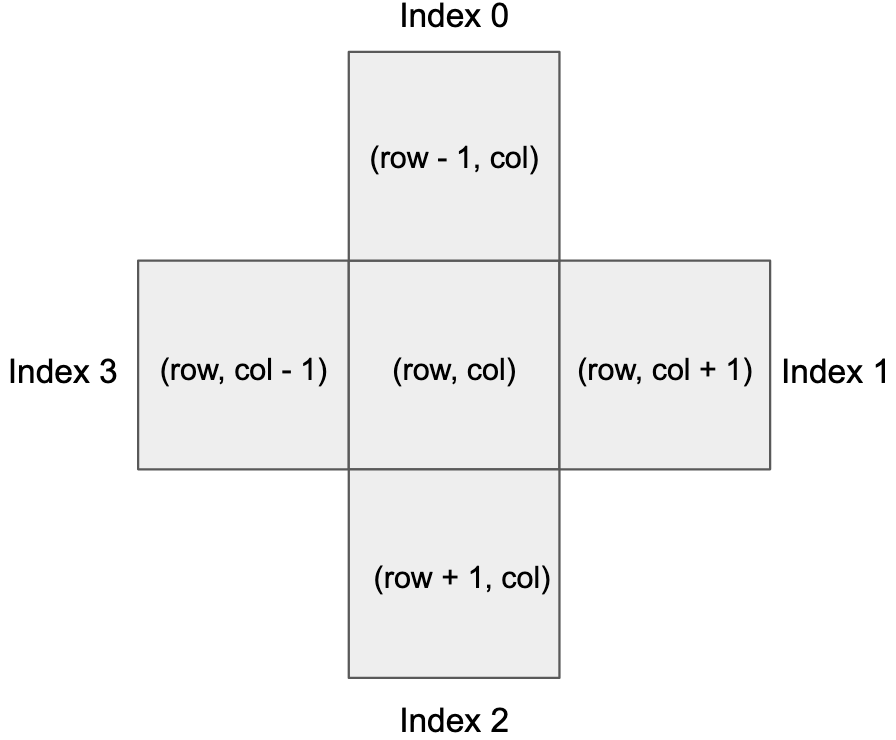
\includegraphics[scale=.45]{calculate_utility_diagram.png}
          % \caption{Example of a parametric plot ($\sin (x), \cos(x), x$)}
        \end{figure}
        \begin{table}[H]
          \begin{center}
            \begin{tabular}{c|c|c}
              \textbf{Intended Action} & \textbf{90$^{\circ}$ Anti-Clockwise Action} & \textbf{90$^{\circ}$ Clockwise Action}\\
              \hline
              North (index 0) & West (index 3) & East (index 1)\\
              East (index 1) & North (index 0) & South (index 2)\\
              South (index 2) & East (index 1) & West (index 3)\\
              West (index 3) & South (index 2) & North (index 0)\\
            \end{tabular}
            \caption{Possible actions undertaken due to probability depending on intended action.}
            \label{tab:table1}
          \end{center}
        \end{table}
        From looking at the diagram and the table, you can now work out any possible action from an intended action using indices. To get the index of the position which is 90$^{\circ}$ anti-clockwise to the intended action, you need to add 3 to the corresponding index to your action, mod 4 and to get the position which 90$^{\circ}$ clockwise to the intended action, you need to add 1 to the corresponding index to your action, mod 4.
        \newline \newline
        Now that you know all coordinates that are associated when making a certain move, you multiply the value of the position that you will end up when making the intended action by 0.8 and the value of the positions if you make an action 90$^{\circ}$ to the intended action by 0.1. After, place the sum of the values in a tuple with the intended action and add it to the `prob' list. When calculations are done for all possible actions, return the `prob' list.
        \newline \newline
        The `value\_iteration' only takes the first element of each tuple in the list returned by `calculate\_expected\_utility', which is the expected utility for each intended action. The maximum expected utility is calculated and this value is inputted in the Bellman's equation, in which the answer is then assigned as the utility of that position on the board.
        \newline \newline
        We then calculate the total difference between the previous board and the new board in terms of utilities. If the total is less than the threshold, then the difference is so small that iterating through the board again is obsolete, therefore we break. However, if the total difference between the two boards is larger than the threshold, then we depreciate the variable `iterations' by 1 and loop through the new board. When `iterations' is equal to zero or when we break from the loop, the new board calculated is returned to `getAction', where `getAction' then calls on `calculate\_expected\_utility' with the current position of the pacman and the new board obtained from `value\_iteration' as parameters. This will then allow the returning of an action that has the maximum expected utility, if only the action is legal.

      \section*{Creativity}
        \begin{itemize}
          \item Identifying positions that are at a right angle to the current position by manipulating indicies using addition and modulus. This avoids the need to have many if statements for every action. In `calculate\_expected\_utility, only one if statement was used.
          \item Setting the reward of the positions that surround the ghosts to a value that is larger than the ghost reward but less than the non-terminal reward. This is essentially a warning to the pacman that going in that direction means they will be closer to the ghost.
          \item Used threshold and a limit to how many iterations you have to loop through the board. Prevents value\_iteration from running infinitely and if the difference is small enough, does not waste computational power and time to iterate again.
        \end{itemize}


      \section*{Performance Analysis}

        \begin{table}[H]
          \begin{center}
            \begin{tabular}{c|c|c}
              \textbf{No. of Iterations} & \textbf{Small Grid Win Rate (\%)} & \textbf{Medium Classic Win Rate (\%)}\\
              \hline
              % 80, 73, 78
              % 84, 80, 80, 84 - 85.6
              % 88, 86, 84, 84 - 85.6
              10 & 100.0 & 82.0 \\ % 77, 86, 83, 78, 86
              11 & 100.0 & 85.6 \\  % 80, 88, 89, 90, 81
              12 & 100.0 & 83.0 \\ % 83, 79, 80, 89, 84
              13 & 100.0 & 81.6 \\ % 81.5, 85, 80, 80
              14 & 100.0 & 85.0 \\ % 83, 89, 83, 86, 84
              15 & 100.0 & 86.0\\ % 90, 87, 87, 86, 80,
              16 & 100.0 & 87.0\\ % 178, 86, 83, 88
              17 & 100.0 & 89.8\\ % 184, 84, 90, 91
              18 & 100.0 & 86.2\\ % 86, 84, 90, 82, 89
              19 & 100.0 & 90.0\\ % 2
              20 & 100.0 & 89.0\\ % 2
            \end{tabular}
            \caption{Finding optimum number of iterations which results in highest win rate. For each iteration, the game was run 500 times \& $\gamma$ = 0.9.}
            \label{tab:table5}
          \end{center}
        \end{table}

        \begin{figure}[H]
          \centering
          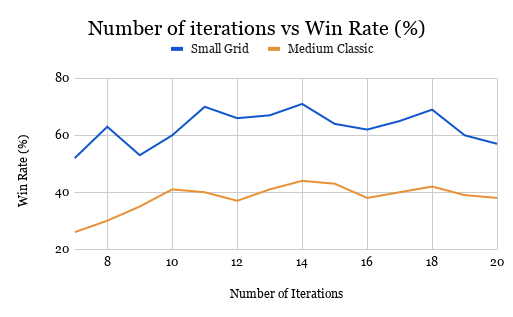
\includegraphics[scale=.45]{iterations_graph.png}
          \caption{Graph showing relationship between number of iterations and win rate for each layout}
        \end{figure}
        Starting point for number of iterations was initially 1, however the average win rate for medium class was 14\% and it runs possibly infinitely for small grid. Therefore, it was realised that the starting point needs to be considerably higher, thus 10 was chosen as the official starting point.
        \begin{table}[h!]
          \begin{center}
            \begin{tabular}{c|c|c}
              \textbf{Board} & \textbf{Win Rate} & \textbf{Average Win Rate (\%)} \\
              \hline
              SMALL GRID & 377/500 & 75.4\\
              MEDIUM CLASSIC & 279/500 & 55.8\\
            \end{tabular}
            \caption{Win rate for the two boards. Used set amount of iterations (10) \& $\gamma$ = 0.9.}
            \label{tab:table2}
          \end{center}
        \end{table}

        \begin{table}[h!]
          \begin{center}
            \begin{tabular}{c|c|c}
              \textbf{Board} & \textbf{Win Rate} & \textbf{Average Win Rate (\%)} \\
              \hline
              SMALL GRID & 382/500 & 76.4\\
              MEDIUM CLASSIC & 279/500 & 55.8\\
            \end{tabular}
            \caption{Win rate for the two boards. Used a threshold of 0.01 \& $\gamma$ = 0.9.}
            \label{tab:table3}
          \end{center}
        \end{table}

        \begin{table}[h!]
          \begin{center}
            \begin{tabular}{c|c}
              \textbf{} & \textbf{Average Win Rate (\%)} \\
              \hline
              WITHOUT THRESHOLD & 57.2\\
              WITH THRESHOLD & 60\\
            \end{tabular}
            \caption{Win rate when causing ghosts' rewards to be -0.04 when scared and -3 when not scared. 10 iterations \& $\gamma$ = 0.9.}
            \label{tab:table4}
          \end{center}
        \end{table}

          The choice was to keep the ghosts' rewards constant throughout the game was made due to the fact that it takes a shorter time to compute the final action to take and on average, the win rate is high compared to tailoring the ghosts' rewards based on if they were scared or not.




  \section*{Conclusion}
  none

\end{document}

% As  you  work  through  your  implementation  of  the  MDP-solver,  you  will  find  that  you  are  makinglots  of  decisions  about  how  precisely  to  translate  your  ideas  into  working  code.  The  report  should explain  these  at  length.
% The  perfect  report  will  give  enough  detail  that  we  don’t  feel  we  have  to read your code in order to understand what you code does (we will read it anyway).Given  the  requirement  for  your  code  to  be  based  around  an  MDP-solver,  you  would  be  wise  to include a description of how your code solves the MDP, and which bits of the code do this solving.
 % Make sure you highlight these aspects of your work, especially things that make your work unique.
% Your  report  should  also  analyse  the  performance  of  your  code.  Because  there  is  a  certain  amountof  randomness  in  the  behaviour  of  the  ghosts,  a  good  analysis  will  run  multiple  games  to  assessPacman’s performance.  For example, you might like to try running:python pacman.py -n 50 -q -p MDPAgent -l mediumClassicto get a statistically significant number of runs so that you can, for example, establish the averagescore with some accuracy.  (Of course, to decide whether this was a statistically significant number of runs,  you  would  have  to  do  some  statistical  analysis  —  it  might  well  need  more  runs.)  All  the conclusions that you present in your analysis should be justified by the data that you have collected
